\chapter{Introducción general}
\label{Chapter1}

En este capítulo se presenta el contexto general del trabajo desarrollado y se introducen los conceptos fundamentales relacionados con los sistemas embebidos aplicados a automatización industrial. Se describe la motivación del trabajo, se revisan las principales tecnologías existentes y se establecen los objetivos definidos para el desarrollo del sistema propuesto.

%----------------------------------------------------------------------------------------

\section{Automatización industrial}

La automatización industrial constituye uno de los pilares fundamentales de los sistemas de producción modernos, ya que permite incrementar la eficiencia, confiabilidad y trazabilidad de los procesos industriales mediante la incorporación de tecnologías de monitoreo, control y comunicación \cite{future_industrial_communication}. En el contexto de la Industria 4.0, la integración de dispositivos inteligentes, redes de comunicación y sistemas distribuidos adquirió un rol central en el desarrollo de arquitecturas industriales flexibles y altamente interconectadas \cite{future_industrial_communication,communication_technology_i40}.

Dentro de este escenario, los sistemas embebidos representan un componente esencial de las plataformas de automatización modernas \cite{shylla2023embedded}. Estos sistemas permiten integrar capacidades de adquisición de datos, procesamiento, comunicación y control en dispositivos compactos y especializados, lo que posibilita la implementación de soluciones orientadas a monitoreo de variables de proceso, supervisión remota, control de actuadores y adquisición distribuida de datos.

En paralelo, la evolución de los microcontroladores modernos y de los sistemas operativos de tiempo real permitió desarrollar sistemas embebidos cada vez más complejos y conectados \cite{overview_embedded_i40}. Actualmente, es posible integrar múltiples interfaces de comunicación y ejecutar tareas concurrentes en tiempo real mediante dispositivos de bajo consumo y reducido tamaño. Asimismo, la utilización de arquitecturas de software modulares y protocolos de comunicación estandarizados facilita la interoperabilidad entre dispositivos y la adaptación de una misma plataforma a diferentes aplicaciones industriales \cite{overview_embedded_i40,communication_technology_i40}.

En este contexto, los sistemas embebidos aplicados a automatización industrial constituyen una herramienta fundamental para el desarrollo de soluciones distribuidas de monitoreo y control. Su utilización permite implementar plataformas flexibles y escalables capaces de integrar procesamiento local, comunicación y supervisión en tiempo real dentro de distintos entornos industriales. Además, las arquitecturas distribuidas y las redes inalámbricas industriales representan una alternativa de creciente interés en aplicaciones asociadas a fábricas inteligentes y sistemas de manufactura avanzados \cite{review_iwn_industry40}.

La figura \ref{fig:red_control_distribuida} presenta un ejemplo conceptual de una arquitectura distribuida de monitoreo y control industrial, compuesta por una estación central, múltiples estaciones remotas y dispositivos de campo interconectados mediante enlaces de comunicación.

\begin{figure}[ht]
	\centering
	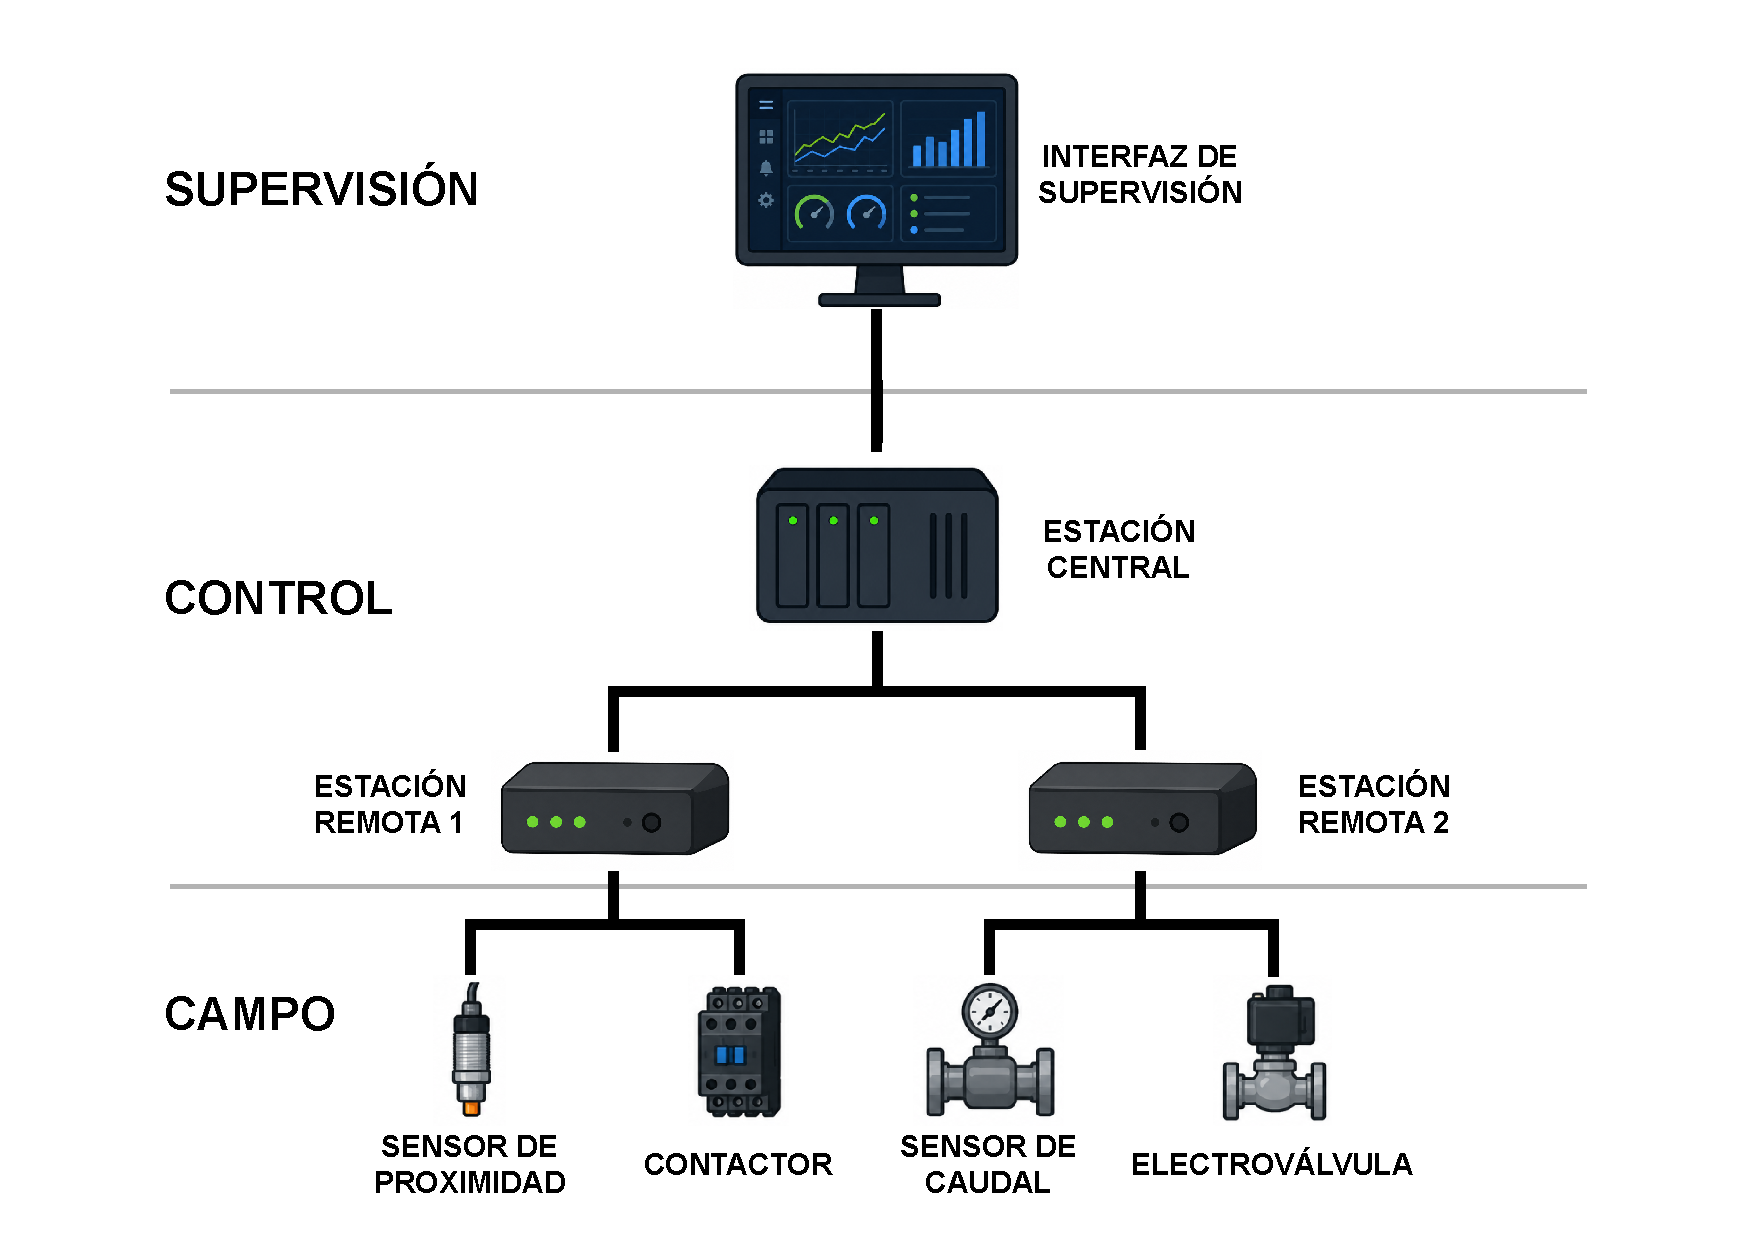
\includegraphics[scale=.4]{./Figures/red_control_distribuida.pdf}
	\caption{Arquitectura de un sistema distribuido de monitoreo y control industrial.}
	\label{fig:red_control_distribuida}
\end{figure}

%----------------------------------------------------------------------------------------

\section{Contexto y motivación}

Tradicionalmente, gran parte de los sistemas de automatización industrial se implementaron mediante arquitecturas centralizadas y redes cableadas. Si bien estas soluciones ofrecen altos niveles de robustez y confiabilidad, también presentan limitaciones en entornos donde el tendido de cables resulta costoso, complejo o poco práctico \cite{review_iwn_industry40}. Esta situación es frecuente en pequeñas y medianas industrias, instalaciones distribuidas geográficamente o procesos que requieren modificaciones frecuentes en la disposición física de los equipos.

En estos escenarios, la incorporación de tecnologías de comunicación inalámbrica permite aumentar la flexibilidad de instalación y reducir significativamente los costos asociados a infraestructura \cite{review_iwn_industry40}. Además, las arquitecturas distribuidas facilitan la expansión del sistema mediante la incorporación de nuevos nodos sin necesidad de realizar modificaciones importantes en el cableado existente.

Dentro de este contexto, los sistemas distribuidos de monitoreo y control representan una alternativa de creciente interés para aplicaciones industriales. Estas arquitecturas se basan en la utilización de una estación central y múltiples nodos remotos capaces de interactuar con sensores y actuadores ubicados en distintos puntos de una planta o instalación \cite{review_iwn_industry40}. La información recolectada puede transmitirse hacia sistemas de supervisión o control, lo que permite centralizar el monitoreo del proceso y mejorar la capacidad de diagnóstico y mantenimiento.

La motivación principal del presente trabajo surge de la necesidad de desarrollar una plataforma embebida flexible, escalable y de bajo costo de implementación, orientada a aplicaciones de monitoreo y control industrial distribuido. El sistema propuesto busca integrar capacidades de adquisición de señales, control de entradas y salidas, procesamiento local y comunicación entre nodos, utilizando una arquitectura modular que facilite su adaptación a diferentes escenarios de aplicación \cite{overview_embedded_i40}. Particularmente, se busca ofrecer una solución técnicamente viable para pequeñas y medianas industrias, donde los costos asociados a infraestructura y expansión suelen representar una limitación significativa para la incorporación de tecnologías de automatización.

%----------------------------------------------------------------------------------------

\section{Estado del arte}

La evolución de los sistemas de automatización industrial dio lugar al desarrollo de diversas tecnologías de comunicación destinadas a satisfacer los requerimientos de monitoreo y control de los procesos productivos. En la actualidad conviven soluciones cableadas e inalámbricas, cada una con características particulares en términos de desempeño, flexibilidad y costo de implementación. A continuación, se revisan las tecnologías más representativas relacionadas con la propuesta desarrollada en el presente trabajo.

\subsection{Redes industriales cableadas}

En los entornos de automatización industrial modernos, las redes de comunicación constituyen un elemento fundamental para la adquisición de datos, supervisión y control de procesos. Tradicionalmente, la industria ha adoptado soluciones cableadas debido a su elevada confiabilidad, inmunidad al ruido electromagnético y capacidad para garantizar tiempos de comunicación determinísticos \cite{future_industrial_communication,communication_technology_i40}.

Las redes industriales cableadas permiten la interconexión de sensores, actuadores, PLC (\textit{Programmable Logic Controller}, Controlador Lógico Programable) y sistemas de supervisión industrial, lo que posibilita el intercambio de información en tiempo real dentro de plantas y procesos automatizados. Entre las tecnologías más utilizadas se destacan buses de campo y soluciones basadas en Ethernet industrial, como PROFIBUS y PROFINET, ampliamente adoptadas en aplicaciones de automatización industrial \cite{profibus_official,profinet_official}.

La evolución de los sistemas industriales y la aparición de los conceptos de Industria 4.0 e IIoT (\textit{Industrial Internet of Things}, Internet Industrial de las Cosas) impulsaron además la integración de infraestructuras Ethernet, sistemas distribuidos y arquitecturas orientadas a comunicaciones en tiempo real \cite{future_industrial_communication}. Sin embargo, a pesar de sus ventajas en términos de robustez y desempeño, las soluciones cableadas presentan limitaciones asociadas a los costos de instalación, mantenimiento y expansión de infraestructura física, especialmente en aplicaciones distribuidas, móviles o de difícil acceso.

\subsection{Redes industriales inalámbricas}

En los últimos años, el avance de los conceptos de Industria 4.0 e IIoT impulsó el crecimiento de las redes inalámbricas industriales como complemento de las infraestructuras cableadas tradicionales \cite{review_iwn_industry40}. Estas tecnologías permiten reducir costos de instalación, simplificar tareas de mantenimiento y aumentar la flexibilidad de despliegue \cite{emerson_wireless,phoenix_trusted_wireless,scalance_wireless}.

Las redes inalámbricas industriales resultan particularmente atractivas para aplicaciones de monitoreo, adquisición distribuida de datos y automatización, debido a ventajas como la movilidad, la facilidad de expansión y la reducción del cableado físico \cite{review_iwn_industry40}. No obstante, los entornos industriales presentan desafíos significativos asociados a interferencias electromagnéticas, obstáculos físicos, topologías dinámicas y requisitos estrictos de latencia y confiabilidad, lo que impone exigencias adicionales sobre los protocolos de comunicación inalámbrica \cite{review_iwn_industry40}.

Gran parte de las soluciones inalámbricas industriales modernas \cite{wirelesshart_official,isa_official,zigbee_official} se basan en el estándar IEEE 802.15.4 \cite{ieee_standard}. Dicho estándar define las capas física PHY (\textit{Physical Layer}) y de control de acceso al medio MAC (\textit{Medium Access Control}) para redes inalámbricas personales de baja velocidad LR-WPAN (\textit{Low-Rate Wireless Personal Area Network}, Red Inalámbrica Personal de Baja Velocidad) \cite{ieee_standard}. Este estándar se caracteriza por su bajo consumo energético, baja complejidad y reducido costo de implementación, características que favorecieron su adopción en sistemas embebidos, redes de sensores inalámbricos e IoT (\textit{Internet of Things}, Internet de las Cosas) \cite{overview_embedded_i40}. Asimismo, múltiples protocolos industriales inalámbricos utilizan IEEE 802.15.4 como base tecnológica para la implementación de mecanismos de comunicación orientados a monitoreo y automatización industrial.

\subsection{Protocolos inalámbricos basados en IEEE 802.15.4}

Entre los protocolos inalámbricos industriales más difundidos basados en IEEE 802.15.4 se encuentra WirelessHART \cite{wirelesshart_official}, ampliamente utilizado en automatización de procesos. Este protocolo incorpora topologías de red mallada (mesh), mecanismos redundantes de comunicación y sincronización temporal, lo que permite aumentar la confiabilidad de la red frente a interferencias o fallas de enlace.

Otra tecnología relevante es ISA100.11a \cite{isa_official,review_iwn_industry40}, diseñada específicamente para aplicaciones industriales de monitoreo y control inalámbrico, con foco en interoperabilidad, escalabilidad y coexistencia con otras tecnologías de comunicación \cite{review_iwn_industry40}.

Zigbee \cite{zigbee_official,review_iwn_industry40} representa otra de las implementaciones más conocidas sobre IEEE 802.15.4. Aunque su adopción se concentra principalmente en aplicaciones IoT, domótica y monitoreo de bajo consumo, muchas de sus características técnicas, como el bajo costo, el soporte para topologías mesh y el reducido consumo energético, lo convierten en una referencia importante dentro del ecosistema de redes inalámbricas embebidas \cite{review_iwn_industry40}.

\subsection{Comparación de soluciones existentes}
La tabla \ref{tab:comparacion_tecnologias} presenta una comparación general entre algunas de las principales tecnologías de comunicación industrial utilizadas en aplicaciones de automatización y monitoreo. Se consideran características relacionadas con el medio de transmisión, las capacidades de tiempo real, el modelo de licenciamiento y el costo de implementación, incluyendo además la propuesta desarrollada en el presente trabajo.

\begin{table}[h]
	\centering
	\caption[Comparación de tecnologías industriales]{Comparación de tecnologías industriales.}
	\begin{tabular}{l c c c c}
		\toprule
		\textbf{Tecnología} & \textbf{Medio} & \textbf{T. real} & \textbf{Licencia} & \textbf{Costo} \\
		\midrule
		PROFIBUS \cite{profibus_official} & Cableado & Alto & Propietaria & Alto \\
		
		PROFINET \cite{profinet_official} & Cableado & Muy alto & Propietaria & Alto \\
		
		WirelessHART \cite{wirelesshart_official} & Inalámbrico & Medio & Requerida & Alto \\
		
		ISA100.11a \cite{isa_official} & Inalámbrico & Medio & Requerida & Alto \\
		
		Zigbee \cite{zigbee_official} & Inalámbrico & Bajo & Parcialmente abierta & Medio \\
		
		Propuesta & Inalámbrico & Medio & Propia & Bajo \\
		\bottomrule
		\hline
	\end{tabular}
	\label{tab:comparacion_tecnologias}
\end{table}

La solución propuesta en este trabajo toma como referencia las arquitecturas inalámbricas industriales modernas basadas en IEEE 802.15.4, priorizando una implementación flexible, modular y de bajo costo orientada a aplicaciones embebidas de monitoreo y control distribuido. El desarrollo busca proporcionar una plataforma adaptable a distintos procesos productivos, capaz de integrarse con sensores y actuadores industriales mediante una arquitectura escalable y reutilizable. Asimismo, se plantea como una alternativa de bajo costo de implementación orientada a pequeñas y medianas industrias, donde las limitaciones económicas y de infraestructura suelen dificultar la incorporación de soluciones convencionales de automatización industrial.

%----------------------------------------------------------------------------------------

\section{Objetivos del trabajo}

Los objetivos definidos para el presente trabajo establecen el propósito general del sistema desarrollado y delimitan las principales actividades necesarias para su diseño, implementación y validación. A continuación, se presentan el objetivo general y los objetivos específicos que guiaron el desarrollo del proyecto.

\subsection{Objetivo general}
Desarrollar un sistema embebido modular y escalable orientado a aplicaciones de monitoreo y control industrial distribuido, basado en una arquitectura compuesta por una estación central y múltiples estaciones remotas interconectadas mediante comunicación inalámbrica \cite{proyecto}.

\subsection{Objetivos específicos}
Los objetivos específicos definidos para el desarrollo del presente trabajo son los siguientes \cite{proyecto}:

\begin{itemize}
	\item Diseñar e implementar un prototipo funcional de estación central basado en un microcontrolador de altas prestaciones capaz de ejecutar un sistema operativo de tiempo real RTOS (\textit{Real-Time Operating System}, Sistema Operativo de Tiempo Real).
	
	\item Diseñar e implementar prototipos funcionales de estaciones remotas con capacidad de adquisición de señales y control de entradas y salidas industriales.
	
	\item Implementar un sistema de comunicación inalámbrica entre estaciones utilizando tecnología basada en IEEE 802.15.4.
	
	\item Desarrollar el firmware necesario para la inicialización y gestión de periféricos, comunicaciones y manejo de entradas y salidas en las estaciones central y remotas.
	
	\item Diseñar una arquitectura de software modular que permita abstraer las dependencias de hardware y facilite la reutilización y escalabilidad del sistema.
	
	\item Implementar interfaces de conexión para sensores y actuadores industriales que permitan adaptar el sistema a diferentes aplicaciones de monitoreo y control.
	
	\item Diseñar e implementar la arquitectura de alimentación de las estaciones.
	
	\item Validar el funcionamiento del sistema mediante pruebas experimentales orientadas a verificar la comunicación entre nodos, el procesamiento de señales y el control de entradas y salidas.
	
\end{itemize}
